% Created 2021-01-24 Sun 22:49
% Intended LaTeX compiler: pdflatex
\documentclass[11pt]{article}
\usepackage[utf8]{inputenc}
\usepackage[T1]{fontenc}
\usepackage{graphicx}
\usepackage{grffile}
\usepackage{longtable}
\usepackage{wrapfig}
\usepackage{rotating}
\usepackage[normalem]{ulem}
\usepackage{amsmath}
\usepackage{textcomp}
\usepackage{amssymb}
\usepackage{capt-of}
\usepackage{hyperref}
\usepackage{minted}
\hypersetup{colorlinks=true, linkcolor=black, filecolor=red, urlcolor=blue}
\usepackage[turkish]{babel}
\author{Eren Hatırnaz}
\date{19 Ocak 2020}
\title{Yazılım Gündemi - 2020/03\\\medskip
\large 13-19 Ocak 2020}
\hypersetup{
 pdfauthor={Eren Hatırnaz},
 pdftitle={Yazılım Gündemi - 2020/03},
 pdfkeywords={},
 pdfsubject={},
 pdfcreator={Emacs 27.1 (Org mode 9.3)},
 pdflang={Turkish}}
\begin{document}

\maketitle
\tableofcontents \clearpage\shorthandoff{=}

\begin{center}
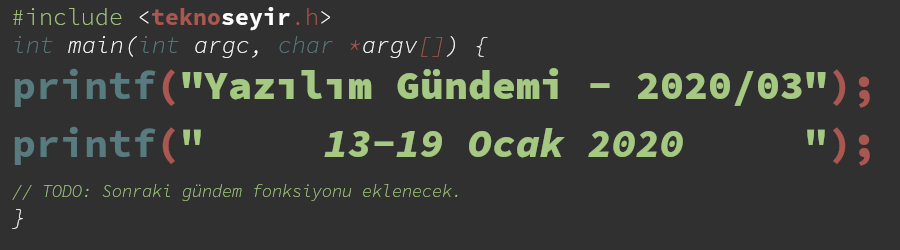
\includegraphics[width=.9\linewidth]{gorseller/yazilim-gundemi-banner.png}
\end{center}

\begin{center}
\href{../02/yazilim-gundemi-2020-02.pdf}{< Önceki Gündem} | \textbf{13-19 Ocak 2020} | \href{../04/yazilim-gundemi-2020-04.pdf}{Sonraki Gündem >}

\href{https://teknoseyir.com/blog/yazilim-gundemi-2020-03}{TeknoSeyir'de Oku}
\end{center}

\section{Git 2.25 \href{https://lore.kernel.org/git/xmqqtv4zjgv5.fsf@gitster-ct.c.googlers.com/}{sürümü duyuruldu}}
\label{sec:org16ca78a}
Versiyon kontrol sistemleri krallığının tahtında oturmaya devam eden Git, bu
hafta içerisinde 2.25 sürümünü çıkardı. Birkaç özelliği birlikte inceleyelim:
\subsection{\href{https://git-scm.com/docs/git-sparse-checkout}{git sparse-checkout} ile parçalı depo indirme}
\label{sec:org3db7648}
2019 yılı boyunca en çok konuşulan kavramlardan biri de mono-repo yapısı
olmuştur sanırım. Bilmeyenler için kısaca açıklayalım: Mono-repo, projenin
belirli parçalarının ayrı depolarda (repository) tutulması yerine hepsinin tek
bir depoda toplanması durumudur. Atıyorum bir not tutma uygulaması
yapıyorsunuz, bu uygulamanın iOS, Android, Web ve masaüstü tüm istemcilerinin
kodları tek bir repository üzerinde duruyor. Çok fazla araştırmadığım ve hiç
kullanmadığım için faydalarını tam bilmiyorum fakat bu yapıyı kullanan büyük
şirketlerin olduğunu biliyorum.

Mono-repo yapısındaki bir depoyu indirmenin ne kadar zaman alabileceğini
tahmin ediyorsunuzdur. İşte Git'in bu sürümünde eklenen \texttt{sparse-checkout}
komutu da tam olarak bu tarz büyük depolarda kullanılması için tasarlanmış.
Tüm depoyu indirmek yerine sadece belirlediğiniz dosya yolundaki dosyaları
indirip, diğerlerini görmezden gelebiliyorsunuz. Henüz deneysel olan bu
özelliği destekleyen pek uzak git sunucusu yok ama yine de biz bir bakalım. Bu
özelliği kullanmak için:

\begin{verbatim}
$ git clone --filter=blob:none --no-checkout /sizin/deponuz/ depo
$ cd depo
$ git sparse-checkout init
\end{verbatim}
komutlarını çalıştırmanız yeterli. Sırasıyla çalıştırdığımız komutları
incelemek gerekirse:

İlk komut bildiğimiz clone komutu ama birkaç eklemesi var.
\texttt{-{}-filter=blob:none} eklemesi ile clone komutuna diyoruz ki hiçbir dosyayı
indirme. Bu parametrenin kabul ettiği başka filtreleme özellikleri de mevcut.
Örneğin \texttt{-{}-filter=blob:10m} parametresi ile 10MB'dan büyük dosyaları indirme
diyebiliyoruz. Diğer filtreleme özellikleri için \href{https://github.com/git/git/blob/v2.25.0/Documentation/rev-list-options.txt\#L735-L780}{buradaki dokümanı}
inceleyebilirsiniz. Bir diğer ekleme olan \texttt{-{}-no-checkout} parametresi ile de
Git'e sunucudan cevap gelince dosyaları indirme dememiz gerekiyor. Çünkü biz
sparse-checkout yapacağız. Bir sonraki komutla zaten depo klasörümüzün içine
giriyoruz ve sonrasında ise \texttt{sparse-checkout} özelliğini \texttt{init} yaparak
başlatıyoruz. Aynı zamanda \texttt{sparse-checkout} komutunun \texttt{set}, \texttt{list},
\texttt{enable}, \texttt{disable} gibi alt komutları da mevcut.

\begin{verbatim}
$ git sparse-checkout set /dosya/yolu
\end{verbatim}
gibi bir komut çalıştırarak indirmek istediğiniz dosya yollarını
belirtebilirsiniz. Böylece tüm depoyu indirmek yerine sadece çalışmak
istediğiniz alt projeyi indirebiliyorsunuz.

Bu yeni özellik hakkında GitHub'ın yayınlandığı detaylı bir blog yazısı
mevcut. Komutun tarihçesi ve detayları için \href{https://github.blog/2020-01-17-bring-your-monorepo-down-to-size-with-sparse-checkout/}{bu bağlantıya} tıklayabilirsiniz.

Bu sürümde gelen diğer özellik ve değişiklikler için konu başlığına eklediğim
bağlantıya tıklayabilirsiniz.
\section{Chromium takımı User-Agent bilgilerini \href{https://groups.google.com/a/chromium.org/forum/m/\#!msg/blink-dev/-2JIRNMWJ7s/yHe4tQNLCgAJ}{dondurmak istiyor}}
\label{sec:org571efc3}
Google tarafından geliştirilen Chrome tarayıcının açık kaynak olan hali
Chromium tarayıcısının geliştirici takımı bu hafta yayınladıkları doküman ile
Chromium'daki User-Agent bilgilerinin \texttt{deprecate} etme ve dondurma niyetlerini
açıkladılar. Dokümanda yazana göre bu User-Agent bilgileri hem artık gereksiz
uzun string ifadelere dönüşmüş hem de bazı web sitelerinin bu bilgileri
kullanarak kullanıcıları tanıdıkları için bu ifadelerin artık hayatımızdan
çıkma zamanının geldiğini savunuyorlar. Bu User-Agent bilgisi genelde
kullanıcıların hangi tarayıcı ve işletim sistemini kullandıklarını tespit etmek
ve ona göre sitede uyarılar göstermek için kullanılıyor. Bu nedenden dolayı
tarayıcının içerisinden tamamen silemezler ama bu yapının yerine \href{https://wicg.github.io/ua-client-hints/}{User Agent
Client Hints (UA-CH)} isimli yeni bir yapı getirmeyi planlıyorlar. Bu yeni
yapıda artık bir web sitesi, kullanıcının tarayıcısı ve işletim sistemiyle
ilgili bilgilere hemen erişemeyecek bunun için sunucuya bir istek göndermesi
gerekecek. Üstelik bu istekte de, istediği bilgileri belirtmesi gerekecek.

Özelliğin uygulamaya geçmesi için planladıkları takvimi aynı doküman içerisinde
paylaşmışlar. Ayrıca \href{https://twitter.com/\_scottlow/status/1206831008261132289}{Microsoft Edge}, \href{https://github.com/mozilla/standards-positions/issues/202\#issuecomment-558294095}{Mozilla Firefox} ve \href{https://twitter.com/rmondello/status/943545865204989953}{Safari} gibi tarayıcılar
da bu değişikliği destekliyorlarmış.
\section{GitHub Android uygulamasının \href{https://github.blog/2020-01-14-the-github-for-android-beta-is-here/}{Beta programı duyuruldu}}
\label{sec:orgafb96db}
\begin{center}
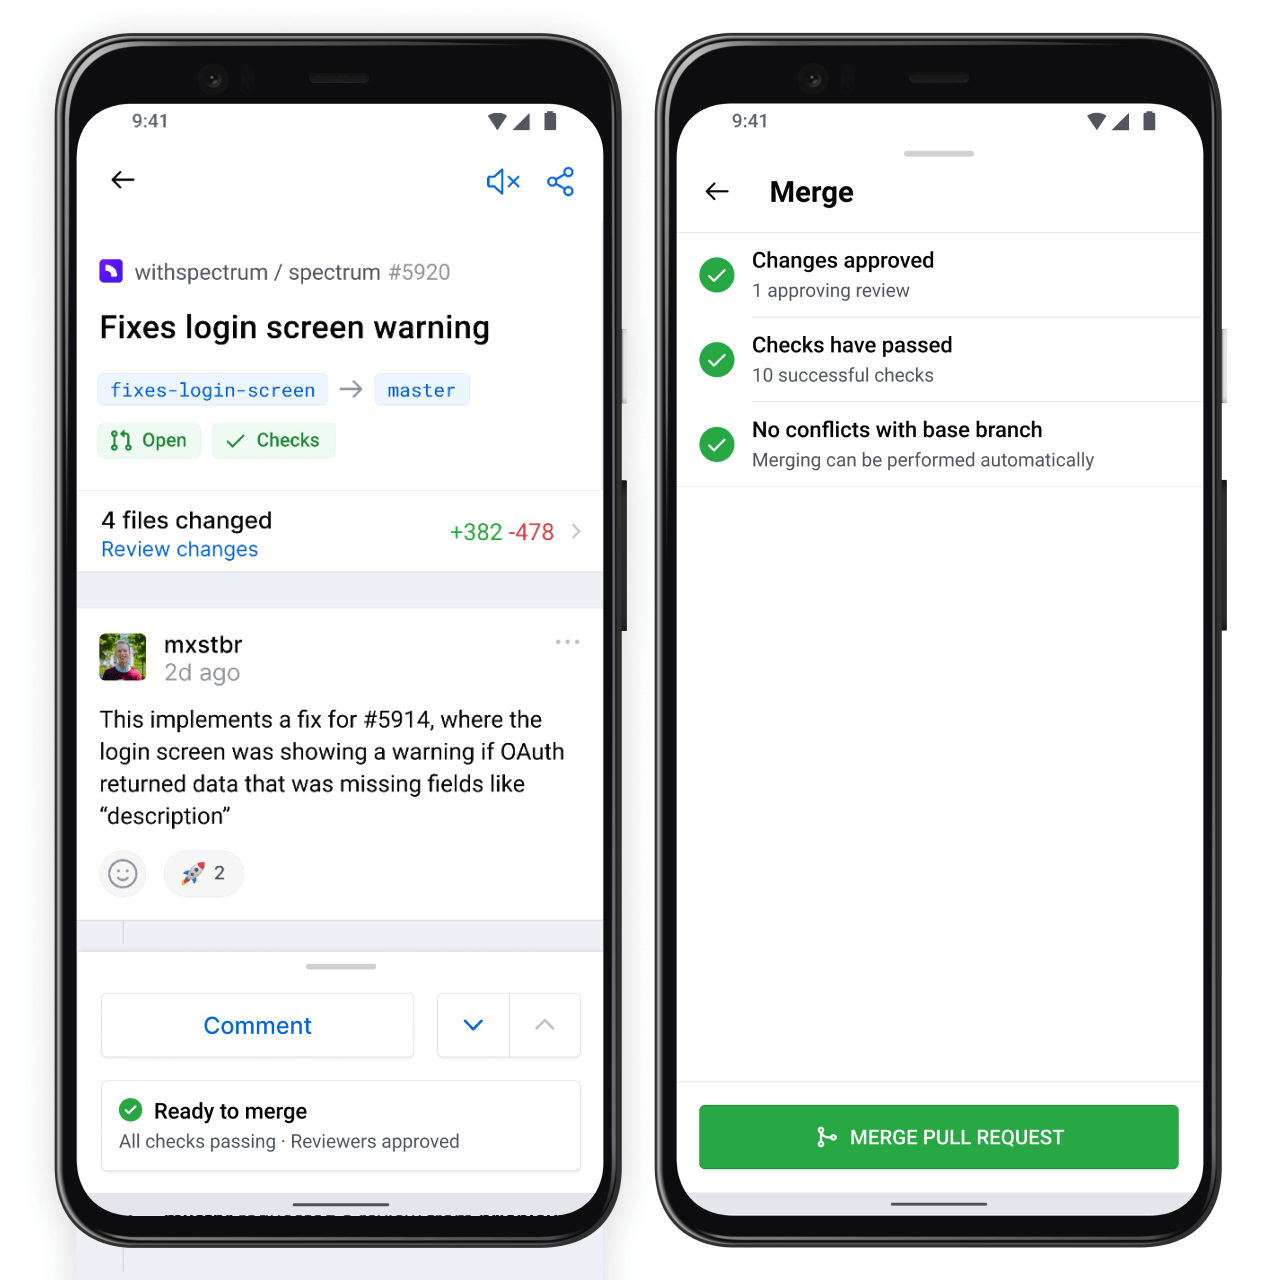
\includegraphics[height=7cm]{gorseller/github-mobil-android.png}
\end{center}

GitHub, Universe 2019 etkinliğinde kendi mobil uygulamalarını tanıtmıştı. Biz
de daha önceki yazılım gündemi yazılarında iOS versiyonunun Beta programının
duyurulduğunu söylemiştik hatta ben Beta programına katılıp uygulamayı
incelemiştim. İlgili yazılım gündemi yazısı için bkz: \href{../../2019/18/yazilim-gundemi-18.pdf}{Yazılım Gündemi - 18}. Bu
hafta da GitHub, Android mobil uygulamasının Beta programını başlattığını
duyurdu. Bende Android telefon olmadığı için başvurup, uygulamayı inceleme
fırsatım olmadı fakat sizler başvurup uygulamayı inceleyip daha sonra da
deneyimlerinizi yorumlar bölümünde paylaşabilirsiniz. Android 5.1 ve üzeri
sürümlerini destekliyor uygulama.

Beta programına katılmak için \href{https://github.com/mobile}{bu sayfayı} ziyaret edebilirsiniz.
\section{JetBrains yazılımcılar için yeni bir \href{https://blog.jetbrains.com/blog/2020/01/15/jetbrains-mono-a-new-font-made-for-developers/}{yazı tipi duyurdu}: \href{https://www.jetbrains.com/lp/mono/}{JetBrains Mono}}
\label{sec:org81167c0}
\begin{center}
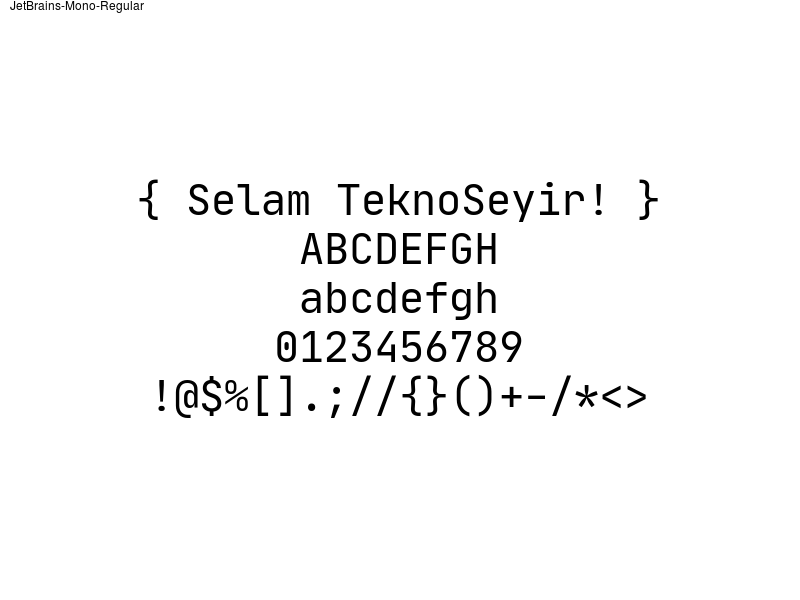
\includegraphics[height=6cm]{gorseller/jetbrains-mono-demo.png}
\end{center}

\href{https://kotlinlang.org/}{Kotlin} programlama dilini geliştiren ve IDE'leri ile meşhur olan sektörümüz
için güzel araçlar üreten \href{https://www.jetbrains.com/}{JetBrains} firması bu sefer de açık kaynak ve ücretsiz
bir yazı tipi ile karşımızda. Kendi geliştirdiği IDE'lerinin son sürümlerinin
hepsinde varsayılan olarak artık bu yazı tipi gelecek. Elbette siz kendi
zevkinize uygun yazı tipiyle değiştirmekte özgürsünüz. Ben de şu an bu yazıyı
yazdığım \href{https://www.gnu.org/software/emacs/}{Emacs} üzerinde JetBrains'in bu yeni yazı tipini deneme amaçlı
kullanıyorum. Hoşuma gitti ve oldukça alıştım. Önceden \href{https://input.fontbureau.com/}{Input Mono} isimli yazı
tipini kullanıyordum fakat bir artık yeni yazı tipim bu olacak gibi gözüküyor.

\begin{center}
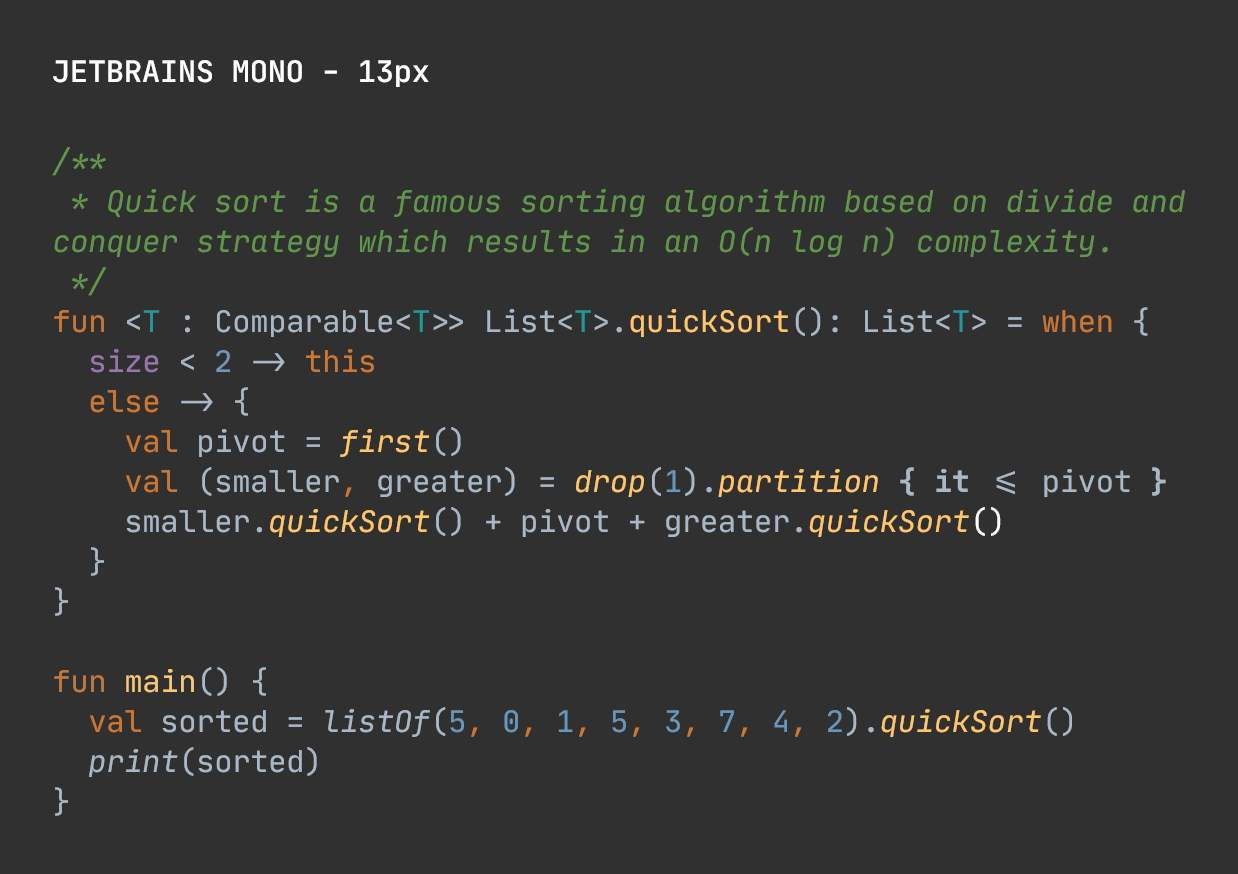
\includegraphics[height=6cm]{gorseller/jetbrains-mono-demo2.png}
\end{center}

Bu yazı tipi aynı zamanda "ligatures" isimli birden çok karakteri tek karakter
gibi gösteren özelliği de destekliyor:

\begin{center}
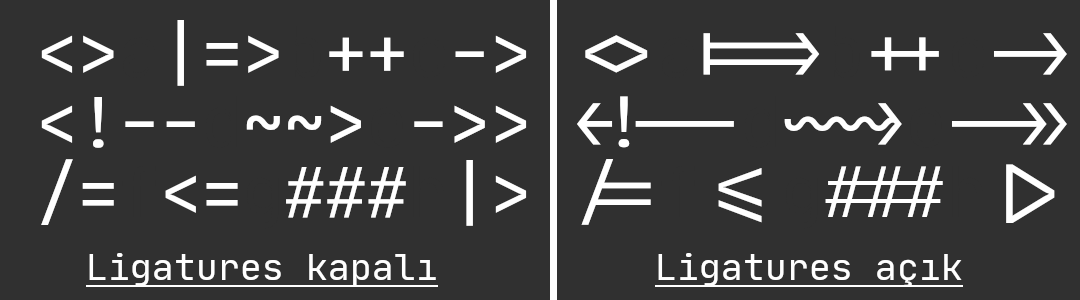
\includegraphics[width=.9\linewidth]{gorseller/jetbrains-mono-ligatures.png}
\end{center}

Sizce yazı tipi nasıl olmuş? Programlama yaparken kullanır mısınız? Siz
programlama yaparken hangi yazı tipini kullanıyorsunuz? Yorumlar bölümünde
konuşalım.

Yeni yazı tipi hakkındaki diğer detaylar için konu başlığına eklediğim
bağlantılara mutlaka tıklayın. JetBrains yine her zaman olduğu gibi harika bir
tanıtım sayfası hazırlamış yazı tipi için.
\section{Windows Terminal Preview v0.8 \href{https://devblogs.microsoft.com/commandline/windows-terminal-preview-v0-8-release/}{duyuruldu}}
\label{sec:org14082c8}
Microsoft'un yaklaşık bir yıldır geliştirmeye devam ettiği terminal
uygulamasının bu hafta v0.9 Preview sürümü duyuruldu. Bu sürüm ile gelen bazı
özellikler ise şu şekilde:
\subsection{Arama}
\label{sec:orgf439f93}
Evet, bildiğimiz düz metin arama özelliği henüz yeni eklenmiş terminal
uygulamasına. Varsayılan olarak CTRL+SHIFT+F tuşları ile kullanılabilir fakat
isterseniz özelleştirebiliyorsunuz tabii ki.

\url{gorseller/windows-terminal-08-arama.gif}
\subsection{Sekme boyutu değiştirme}
\label{sec:orgc678cfc}
Terminal uygulamasında birden fazla sekme içerisinde farklı kabuklar (shell)
çalıştırabiliyorsunuz elbette. Bu sürüm ile birlikte ise bu sekmelerin
boyutlandırma davranışlarını değiştirme özelliği gelmiş. İki farklı değer
verebiliyorsunuz bu özelliğe, İlki: \texttt{equal} (eşit) adı üzerinde tüm sekmelerin
boyutlarını eşit olarak ayarlıyor ve yeni sekmeler açınca hepsini birden aynı
boyutlarda olacak şekilde sıkıştırıyor; ikincisi ise: \texttt{titleLength} (başlık
boyutu) bununla da sekmenin başlığında yazan yazı kadar boyutlandırma
yaptırabiliyorsunuz. Windows Terminal uygulaması varsayılan olarak
\texttt{titleLength} ile gelecek fakat bu davranışı değiştirmek için \texttt{tabWidthMode}
özelliğini özelleştirebilirsiniz.

\url{gorseller/windows-terminal-08-sekme-boyut.gif}

Ayrıca çeşitli retro terminal efektleri gibi oyuncaklar da eklemişler. Diğer
özellikler ve hata gidermeleri için konu başlığına eklediğim bağlantıya
tıklayabilirsiniz.
\section{IntelliJ IDEA 19 yaşında}
\label{sec:org11247c1}
JetBrains firmasının Java geliştirme için ürettiği IntelliJ IDEA IDE'si bu
hafta içerisinde 19.yaşını kutladı. Uzun zamandır Java yazmıyorum, yazdığım
zamanlarda da Eclipse kullanırdım ama yine de IntelliJ IDEA'nın yeni yaşını
kutlamış olalım. Nice mutlu senelere :)

\begin{itemize}
\item \href{https://twitter.com/intellijidea/status/1218172414615597061}{Konuyla ilgilili kutlama tweet'i}
\end{itemize}
\newpage
\section{Yaklaşan Etkinlikler}
\label{sec:orge68b26a}
\begin{longtable}{|p{8cm}|l|l|}
\hline
Etkinlik İsmi & Yeri & Tarihi\\
\hline
\endfirsthead
\multicolumn{3}{l}{Önceki sayfadan devam ediyor} \\
\hline

Etkinlik İsmi & Yeri & Tarihi \\

\hline
\endhead
\hline\multicolumn{3}{r}{Devamı sonraki sayfada} \\
\endfoot
\endlastfoot
\hline
\href{https://www.meetup.com/Teknopark-\%25C4\%25B0stanbul-Yaz\%25C4\%25B1l\%25C4\%25B1mc\%25C4\%25B1-Bulu\%25C5\%259Fmalar\%25C4\%25B1/events/267785470/}{Sürdürülebilir Kod Kalitesi (Continuous Code Quality)} & İstanbul & 22 Ocak 12:30\\
\href{https://kommunity.com/izmir-teknoloji-bulusmasi-sohbet/events/izmir-teknoloji-bulusmasi-sohbet}{İzmir Teknoloji Buluşması - Sohbet} & İzmir & 22 Ocak 19:00\\
\href{https://www.meetup.com/S-Data-Science/events/267905267/}{GPU Üzerinde Derin Öğrenmesiz Veri Bilimi} & İstanbul & 23 Ocak 18:30\\
\href{https://www.meetup.com/IBMCloudTR/events/267829562/}{Watson ile Makine Öğrenmesi Modelleri Oluşturma} & İstanbul & 23 Ocak 19:00\\
\href{https://www.meetup.com/istanbul-yapay-zeka-toplulugu/events/267585252/}{Siber Güvenlikte Derin Öğrenme Atölyesi} & İstanbul & 25 Ocak 10:00\\
\href{https://www.meetup.com/GDG-Izmir/events/268014757/}{Flutter ile ilk uygulamanı yaz} & İzmir & 28 Ocak 18:30\\
\href{https://www.meetup.com/rladies-istanbul/events/267636455/}{rstudio::conf(2020) - Watch Party} & İstanbul & 29 Ocak 19:00\\
\href{https://www.meetup.com/trendyol/events/267607677/}{Scaling Architecture Decision Making} & İstanul & 29 Ocak 19:00\\
\href{https://www.meetup.com/\%25C4\%25B0tu-Ar\%25C4\%25B1-Teknokent-Yaz\%25C4\%25B1l\%25C4\%25B1mc\%25C4\%25B1-Bulu\%25C5\%259Fmalar\%25C4\%25B1/events/267877408/}{Yapay Zeka} & İstanbul & 31 Ocak 18:30\\
\hline
\end{longtable}
\section{Diğer Haberler}
\label{sec:org60d6dc7}
\begin{itemize}
\item GitHub Game Off 2019 yarışmasının \href{https://github.blog/2020-01-14-game-off-2019-winners/}{kazananları açıklandı}. Tüm oyunların kaynak
kodları herkese açık.
\item Google, kod yazmadan mobil uygulama geliştirmeye yarayan \href{https://www.appsheet.com/}{AppSheet} \href{https://techcrunch.com/2020/01/14/google-acquires-appsheet-to-bring-no-code-development-to-google-cloud/}{platformunu
satın aldı}. Artık Google Cloud sisteminin bir parçası.
\item GitLab, Cloudflare CDN hizmetine \href{https://about.gitlab.com/blog/2020/01/16/gitlab-changes-to-cloudflare/}{geçiyor}.
\item ASP.NET takımından mobil hamlesi: \href{https://devblogs.microsoft.com/aspnet/mobile-blazor-bindings-experiment/}{Experimental Mobile Blazor Bindings}.
\item PyTorch kütüphanesinin 1.4.0 \href{https://github.com/pytorch/pytorch/releases/tag/v1.4.0}{sürümü yayınlandı}.
\item Vulkan 1.2 \href{https://www.khronos.org/news/press/khronos-group-releases-vulkan-1.2}{sürümünü duyuruldu}.
\item GNU Guile programlama dilinin 3.0.0 \href{https://www.gnu.org/software/guile/news/gnu-guile-300-released.html}{sürümü yayınlandı}.
\item Next.JS kütüphanesinin 9.2 sürümü \href{https://nextjs.org/blog/next-9-2}{duyuruldu}.
\item Go ile yazılmış HTTP yük testi aracı Cassowary, 0.4.0 \href{https://github.com/rogerwelin/cassowary/releases/tag/v0.4.0}{sürümünü yayınladı}.
\item Gerçek zamanlı veritabanı çözümü SapphireDB, 1.2.0 \href{https://github.com/SapphireDb/SapphireDb/releases/tag/1.2.0}{sürümünü yayınladı}.
\item OpenCore 1.1.0 \href{https://github.com/opencorero/opencore/releases/tag/1.1.0}{sürümü çıktı}.
\end{itemize}
\section{Lisans}
\label{sec:org29a820e}
\begin{center}
\begin{center}

\includegraphics[height=1.5cm]{../../../img/CC_BY-NC-SA_4.0.png}
\end{center}

\href{yazilim-gundemi-2020-03.pdf}{Yazılım Gündemi - 2020/03} yazısı \href{https://erenhatirnaz.github.io}{Eren Hatırnaz} tarafından \href{http://creativecommons.org/licenses/by-nc-sa/4.0/}{Creative Commons
Atıf-GayriTicari-AynıLisanslaPaylaş 4.0 Uluslararası Lisansı} (CC BY-NC-SA 4.0)
ile lisanslanmıştır.
\end{center}
\end{document}
